
%(BEGIN_QUESTION)
% Copyright 2009, Tony R. Kuphaldt, released under the Creative Commons Attribution License (v 1.0)
% This means you may do almost anything with this work of mine, so long as you give me proper credit

Suppose the pneumatic tube connecting the I/P to the control valve were to break open at the point shown in this illustration:

$$\includegraphics[width=15.5cm]{i03849x01.eps}$$

Assuming a direct-acting 4-20 mA transmitter (higher speed, more current), a direct-acting I/P transducer (more current, more air pressure), and a controller properly configured for the application, determine what will happen to these variables over time as a result of the tubing break:

\begin{itemize}
\item{} Turbine speed ({\it increase}, {\it decrease}, or {\it no effect})
\vskip 10pt
\item{} 4-20 mA current signal from controller to I/P transducer ({\it increase}, {\it decrease}, or {\it no effect})
\vskip 10pt
\item{} Flow rate of steam into the turbine ({\it increase}, {\it decrease}, or {\it no effect})
\vskip 10pt
\item{} Instrument air supply pressure ({\it increase}, {\it decrease}, or {\it no effect})
\end{itemize}

\underbar{file i03849}
%(END_QUESTION)





%(BEGIN_ANSWER)

\begin{itemize}
\item{} Turbine speed ({\bf decrease})
\vskip 10pt
\item{} 4-20 mA current signal from controller to I/P transducer ({\bf increase})
\vskip 10pt
\item{} Flow rate of steam into the turbine ({\bf decrease})
\vskip 10pt
\item{} Instrument air supply pressure ({\bf no effect} or {\bf decrease})
\end{itemize}

%(END_ANSWER)





%(BEGIN_NOTES)


{\bf This question is intended for exams only and not worksheets!}

%(END_NOTES)


